\documentclass{beamer}
\usepackage[a3,orientation=landscape,scale=3]{beamerposter}

\usepackage[utf8]{inputenc}
\usepackage[spanish]{babel}
\usepackage{amsmath,amssymb,amsthm,amsfonts}
\usepackage{graphicx}

%%%%%%%%%%%%%%%%%%%%%%
\title{Modelos multiagentes}
\author{Augusto Cabrera Becerril}
\date{\today}
\institute{Facultad de Ciencias UNAM}
%\footimage{
\includegraphics[scale=0.2]{p2R.jpeg}}
%%%%%%%%%%%%%%%%%%%%%%
\usetheme{Berlin}
\usecolortheme{}

%%%%%%%%%%%%%%%%%%%%
\begin{document}
\begin{frame}[fragile]
    \begin{columns}[T]
    \begin{column}{0.33\textwidth}
    \begin{block}{Abstract}
       En esta platica  hablaremos de modelos directos de sistemas complejos adaptativos 
    \end{block}
    
    \begin{block}{MBA}
       \begin{itemize}
        \item Agentes
        \item Mundo
        \item Reglas de interaccion
        \end{itemize}
    \end{block}
    \end{column}

    \begin{column}{0.33\textwidth}
        \begin{block}{Imagen}
            
\includegraphics[width=\textwidth]{imagen1.jpg}
        \end{block}
        \begin{block}{ecuaciones}
            El modelo de crecimiento de Malthus consiste en el problema de valores iniciales:

\begin{equation}
    \dot{x}(t)=\kappa x(t)
\end{equation}
con condición inicial $x(0)=X_0$.

 Tiene la solución 
\begin{equation}
    x(t)=X_0\mathrm{e}^{\kappa t}
\end{equation}
        \end{block}
    \end{column}
    \begin{column}{0.31\textwidth}
        \begin{block}{Ejemplo1}
            Modelo valientes y Cobardes
            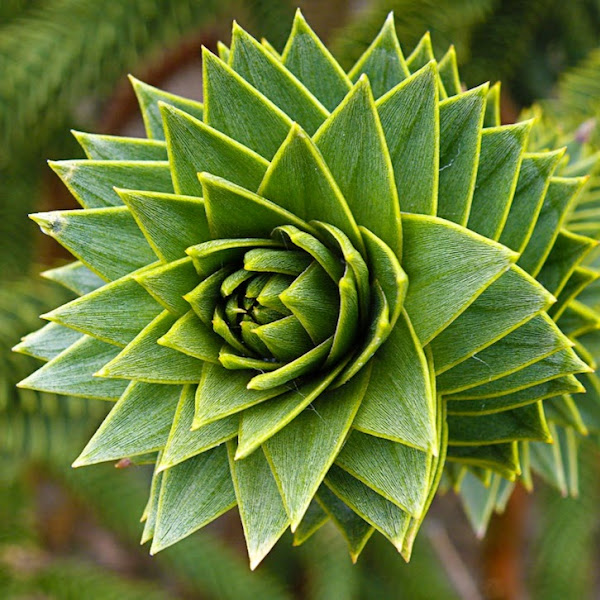
\includegraphics[]{unnamed.jpg}
        \end{block}
        \begin{block}{}
            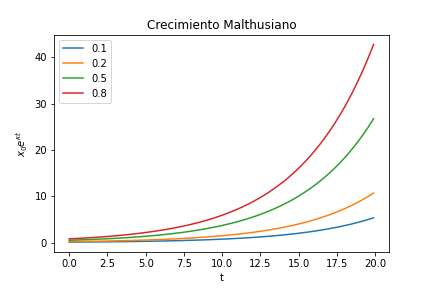
\includegraphics[width=\textwidth]{malthus2.png}
        \end{block}
    
    \end{column}
    
    \end{columns}
\end{frame}
\end{document}
